\documentclass[]{article}
\usepackage{lmodern}
\usepackage{amssymb,amsmath}
\usepackage{ifxetex,ifluatex}
\usepackage{fixltx2e} % provides \textsubscript
\ifnum 0\ifxetex 1\fi\ifluatex 1\fi=0 % if pdftex
  \usepackage[T1]{fontenc}
  \usepackage[utf8]{inputenc}
\else % if luatex or xelatex
  \ifxetex
    \usepackage{mathspec}
  \else
    \usepackage{fontspec}
  \fi
  \defaultfontfeatures{Ligatures=TeX,Scale=MatchLowercase}
\fi
% use upquote if available, for straight quotes in verbatim environments
\IfFileExists{upquote.sty}{\usepackage{upquote}}{}
% use microtype if available
\IfFileExists{microtype.sty}{%
\usepackage{microtype}
\UseMicrotypeSet[protrusion]{basicmath} % disable protrusion for tt fonts
}{}
\usepackage[margin=1in]{geometry}
\usepackage{hyperref}
\hypersetup{unicode=true,
            pdftitle={BAP},
            pdfborder={0 0 0},
            breaklinks=true}
\urlstyle{same}  % don't use monospace font for urls
\usepackage{color}
\usepackage{fancyvrb}
\newcommand{\VerbBar}{|}
\newcommand{\VERB}{\Verb[commandchars=\\\{\}]}
\DefineVerbatimEnvironment{Highlighting}{Verbatim}{commandchars=\\\{\}}
% Add ',fontsize=\small' for more characters per line
\usepackage{framed}
\definecolor{shadecolor}{RGB}{248,248,248}
\newenvironment{Shaded}{\begin{snugshade}}{\end{snugshade}}
\newcommand{\AlertTok}[1]{\textcolor[rgb]{0.94,0.16,0.16}{#1}}
\newcommand{\AnnotationTok}[1]{\textcolor[rgb]{0.56,0.35,0.01}{\textbf{\textit{#1}}}}
\newcommand{\AttributeTok}[1]{\textcolor[rgb]{0.77,0.63,0.00}{#1}}
\newcommand{\BaseNTok}[1]{\textcolor[rgb]{0.00,0.00,0.81}{#1}}
\newcommand{\BuiltInTok}[1]{#1}
\newcommand{\CharTok}[1]{\textcolor[rgb]{0.31,0.60,0.02}{#1}}
\newcommand{\CommentTok}[1]{\textcolor[rgb]{0.56,0.35,0.01}{\textit{#1}}}
\newcommand{\CommentVarTok}[1]{\textcolor[rgb]{0.56,0.35,0.01}{\textbf{\textit{#1}}}}
\newcommand{\ConstantTok}[1]{\textcolor[rgb]{0.00,0.00,0.00}{#1}}
\newcommand{\ControlFlowTok}[1]{\textcolor[rgb]{0.13,0.29,0.53}{\textbf{#1}}}
\newcommand{\DataTypeTok}[1]{\textcolor[rgb]{0.13,0.29,0.53}{#1}}
\newcommand{\DecValTok}[1]{\textcolor[rgb]{0.00,0.00,0.81}{#1}}
\newcommand{\DocumentationTok}[1]{\textcolor[rgb]{0.56,0.35,0.01}{\textbf{\textit{#1}}}}
\newcommand{\ErrorTok}[1]{\textcolor[rgb]{0.64,0.00,0.00}{\textbf{#1}}}
\newcommand{\ExtensionTok}[1]{#1}
\newcommand{\FloatTok}[1]{\textcolor[rgb]{0.00,0.00,0.81}{#1}}
\newcommand{\FunctionTok}[1]{\textcolor[rgb]{0.00,0.00,0.00}{#1}}
\newcommand{\ImportTok}[1]{#1}
\newcommand{\InformationTok}[1]{\textcolor[rgb]{0.56,0.35,0.01}{\textbf{\textit{#1}}}}
\newcommand{\KeywordTok}[1]{\textcolor[rgb]{0.13,0.29,0.53}{\textbf{#1}}}
\newcommand{\NormalTok}[1]{#1}
\newcommand{\OperatorTok}[1]{\textcolor[rgb]{0.81,0.36,0.00}{\textbf{#1}}}
\newcommand{\OtherTok}[1]{\textcolor[rgb]{0.56,0.35,0.01}{#1}}
\newcommand{\PreprocessorTok}[1]{\textcolor[rgb]{0.56,0.35,0.01}{\textit{#1}}}
\newcommand{\RegionMarkerTok}[1]{#1}
\newcommand{\SpecialCharTok}[1]{\textcolor[rgb]{0.00,0.00,0.00}{#1}}
\newcommand{\SpecialStringTok}[1]{\textcolor[rgb]{0.31,0.60,0.02}{#1}}
\newcommand{\StringTok}[1]{\textcolor[rgb]{0.31,0.60,0.02}{#1}}
\newcommand{\VariableTok}[1]{\textcolor[rgb]{0.00,0.00,0.00}{#1}}
\newcommand{\VerbatimStringTok}[1]{\textcolor[rgb]{0.31,0.60,0.02}{#1}}
\newcommand{\WarningTok}[1]{\textcolor[rgb]{0.56,0.35,0.01}{\textbf{\textit{#1}}}}
\usepackage{graphicx,grffile}
\makeatletter
\def\maxwidth{\ifdim\Gin@nat@width>\linewidth\linewidth\else\Gin@nat@width\fi}
\def\maxheight{\ifdim\Gin@nat@height>\textheight\textheight\else\Gin@nat@height\fi}
\makeatother
% Scale images if necessary, so that they will not overflow the page
% margins by default, and it is still possible to overwrite the defaults
% using explicit options in \includegraphics[width, height, ...]{}
\setkeys{Gin}{width=\maxwidth,height=\maxheight,keepaspectratio}
\IfFileExists{parskip.sty}{%
\usepackage{parskip}
}{% else
\setlength{\parindent}{0pt}
\setlength{\parskip}{6pt plus 2pt minus 1pt}
}
\setlength{\emergencystretch}{3em}  % prevent overfull lines
\providecommand{\tightlist}{%
  \setlength{\itemsep}{0pt}\setlength{\parskip}{0pt}}
\setcounter{secnumdepth}{0}
% Redefines (sub)paragraphs to behave more like sections
\ifx\paragraph\undefined\else
\let\oldparagraph\paragraph
\renewcommand{\paragraph}[1]{\oldparagraph{#1}\mbox{}}
\fi
\ifx\subparagraph\undefined\else
\let\oldsubparagraph\subparagraph
\renewcommand{\subparagraph}[1]{\oldsubparagraph{#1}\mbox{}}
\fi

%%% Use protect on footnotes to avoid problems with footnotes in titles
\let\rmarkdownfootnote\footnote%
\def\footnote{\protect\rmarkdownfootnote}

%%% Change title format to be more compact
\usepackage{titling}

% Create subtitle command for use in maketitle
\providecommand{\subtitle}[1]{
  \posttitle{
    \begin{center}\large#1\end{center}
    }
}

\setlength{\droptitle}{-2em}

  \title{BAP}
    \pretitle{\vspace{\droptitle}\centering\huge}
  \posttitle{\par}
    \author{}
    \preauthor{}\postauthor{}
    \date{}
    \predate{}\postdate{}
  
\usepackage{booktabs}
\usepackage{longtable}
\usepackage{array}
\usepackage{multirow}
\usepackage{wrapfig}
\usepackage{float}
\usepackage{colortbl}
\usepackage{pdflscape}
\usepackage{tabu}
\usepackage{threeparttable}
\usepackage{threeparttablex}
\usepackage[normalem]{ulem}
\usepackage{makecell}
\usepackage{xcolor}

\begin{document}
\maketitle

This is an \href{http://rmarkdown.rstudio.com}{R Markdown} Notebook.
When you execute code within the notebook, the results appear beneath
the code.

Background

To accelerate research and decision making data needs to be findable,
accessible, interoperable, and reusable (FAIR). Multiple federal, state
and tribal agencies collect in-stream and riparian habitat metrics to
answer management questions specific to their program goals. This
analysis package integrates data from two different aquatic monitoring
programs; BLM AIM and EPA Rivers and Streams (Table1) . We would like to
integrate two US Forest Service in-stream aquatic habitat monitoring
programs, but their data is not publicity accessible.

Monitoring Program Information

\begin{Shaded}
\begin{Highlighting}[]
\NormalTok{program_info<-(}\KeywordTok{read.xlsx}\NormalTok{(}\StringTok{"Data/Metadata.xlsx"}\NormalTok{, }\DecValTok{1}\NormalTok{))}

\KeywordTok{kable}\NormalTok{(program_info) }\OperatorTok
\StringTok{    }\KeywordTok{kable_styling}\NormalTok{(}\DataTypeTok{bootstrap_options =} \KeywordTok{c}\NormalTok{(}\StringTok{"striped"}\NormalTok{, }\StringTok{"hover"}\NormalTok{, }\DataTypeTok{fixed_header=}\OtherTok{TRUE}\NormalTok{ ))}
\end{Highlighting}
\end{Shaded}

\begin{table}[H]
\centering
\begin{tabular}{l|l|l|l|l}
\hline
Entity & Bureau.of.Land.Management & US.Forest.Service.and.Bureau.of.Land.Management & Environmental.Protection.Agency & US.Forest.Service\\
\hline
Program & Assessment, Inventory, and Monitoring & Aquatic and Riparian Effective Monitoring Program & National Rivers and Streams Assessment & PACFISH/INFISH Biological Opinion Effectiveness Monitoring\\
\hline
Abbreviation & AIM Aquatic & AREMP & NRSA & PIBO EM\\
\hline
Primary Objective & A consistent, quantitative approach for determining the attainment of BLM land health standards for perennial wadeable streams and rivers, among other applications.  Monitoring
objectives are established by project managers and will determine the number of
reaches to be sampled and whether a randomized, targeted, or mixed site
selection approach is appropriate. & Status and Trend & A collaborative survey that provides information on the ecological condition of the nation’s rivers and streams and the key stressors that affect them, both on a national and an ecoregional scale. 
The goals of the NRSA are to determine the extent to which rivers and streams support a healthy biological condition and the extent of major stressors that affect them. The survey supports a longer-term goal: to determine whether our rivers and streams are getting cleaner and how we might best invest in protecting and restoring them. & The primary objective is to determine whether
priority biological and physical attributes, processes, and functions of riparian
and aquatic systems are being degraded, maintained, or restored in the
PIBO monitoring area.\\
\hline
Year Started & 2011 & 2002 & 2008 & 1998\\
\hline
Site Length & 20 x bankfull width, a minimum of 150m & 20x bankfull width categories, range 150m-500m & 20x channel-widths, a minimum of 150m & 20x bankfull channel
widths, range from 160m-480m\\
\hline
Spatial Design & Stratified GRTS, Targeted sites & Non-stratified GRTS & GRTS & GRTS, Targeted sites\\
\hline
Target Population & Surveys conducted in wadeable streams within BLM Bruneau Field Offices & Surveys conducted in wadeable stream within the Northwest Forest Plan Area in Watersheds with at least 25\% of the 1:100K streams layers within federal ownership. & The target population consists of all streams and rivers within the 48 contiguous states that have flowing water during the study index period, including major rivers and small streams. Sites must have > 50\% of the reach length with standing water, and sites with water in less than 50\% of the reach length must be dropped. All sites must be sampled during base flow conditions. The target population excludes:
• Tidal rivers and streams up to head of salt (defined as < 0.5 ppt for this study).
• Run-of-the-river ponds and reservoirs with greater than seven day residence time.
The study index period extends from & Target popultion cosists of 6th fieldhydrologic unit code (HUC) watersheds within perennial streams and greater than 50 percent Federal ownership above the sample reach.\\
\hline
Master Sample Details & Resolution ? & NA & NA & NA\\
\hline
Additional Spatial Design Details & NA & NA & The survey design consists of two separate designs to address the dual objectives of: 
(1)estimating current status and (2) estimating change in status for all flowing waters:
• Resample design applied to NRSA 2008/09 and NRSA 2013/14 sites.
• New site design for NRSA 2018/19.
The survey design is explicitly stratified by state for both designs. The unequal probability categories are specific to the survey design used for the NRSA 2008/09, NRSA 2013/14, and NRSA 2018/19. In all cases the categories are specific combinations of Strahler order categories and nine National Aquatic Resource Survey (NARS) aggregated ecoregions. In addition, a minimum of 20 sites (Resample and New) was guaranteed in each state and a maximum of 75 sites was the limit for an individual state. There are 983 unique sites in the Resample Design and 825 unique sites in the New Site Design. Approximately 10\% of the total NRSA sites are scheduled for repeated sampling (revisit sites) in the same year of the two year NRSA field cycle. The sample frame was derived from the medium resolution National Hydrography Dataset (NHD), in particular NHDPlus V2. Additional details on the NRSA survey design are found in the National Rivers and Streams Assessment Survey Design: 2018/19 documents. & NA\\
\hline
Base Temporal Scale & Annual & Annual & 2008-2009, 2013-2014, 2018-2019 & Annual (5-year rotating panel)\\
\hline
Temporal Design & NA & NA & NA & We will then resample the same watersheds over subsequent 5-year periods. This design is represented as a rotating panel that is serially augmented and alternates over a given period (Urquhart and others 1998). Initially, we will randomly select the subsample of reference and managed watersheds within the group. Our goal will be to select an even number of “reference” and “managed” watersheds for sampling. Because the number of “reference” watersheds is generally low, we will sample as many as possible within the group, up to half of the total number of watersheds.\\
\hline
Sample Period & NA & NA & o Beginning of June through end of September for most regions.
o Sites in the select ecoregions or States can be sampled starting in the end of
April with approval from the EPA Project Coordinator. & NA\\
\hline
Quality Control & Field personnel training, standard protocol & Field personnel training, standard protocol, 9 watersheds are surveyed & Field personnel training, standard protocol & Field personnel training, standard protocol\\
\hline
Protocol & https://aim.landscapetoolbox.org/wp-content/uploads/2018/10/TR\_1735-02.pdf & http://www.reo
.gov/monitoring
/reports/watershed/2010.Field Protocol.Final.pdf & https://www.epa.gov/sites/production/files/2019-05/documents/nrsa\_1819\_fom\_wadeable\_version\_1.2\_0.pdf & https://www.fs.usda.gov/Internet/FSE\_DOCUMENTS/fseprd494543.pdf\\
\hline
Comments & NA & NA & Survey conducted in wadable and bootable streams across the United States. Sampling locations are selected using a modern survey design approach called a probability-based sample design. In such a design, every element in the population has a known probability of being selected for sampling. This important feature ensures that the results of the survey reflect the full range in character and variation among flowing waters across the U.S. Site selection rules included weighting to provide balance in the number of river and stream sites from each of the size classes. & Survey conducted in wadeable streams within the interior ColumbiaRiver basin on lands managed by U.S.orest Service (FS) Regions 1, 4, and 6 and the Idaho and Oregon/Washington State Offices of the Bureau of Land Management (BLM). (AND UPPER MISSOURI? )\\
\hline
Additional References & https://aim.landscapetoolbox.org/wp-content/uploads/2018/01/AIM-strategy011818.pdf & NA & NA & https://www.fs.usda.gov/detail/r4/landmanagement/resourcemanagement/?cid=stelprd3845865\\
\hline
\end{tabular}
\end{table}

Program Metrics

Each monitoring program calculates a standard set of metrics based on
their user's needs. Metadata for the EPA and BLM can be found on their
webpages, PIBO and AREMP is aviable apon request. To facilitate data
sharing we compiled a data dictionary identifing the metrics calculate
by more then one program. You can find the full metric table in !!!!
(NEED TO REVIEW AND PUBLISH) We classified each metirc into a catagory,
table 2 shows the count of metrics by catagory.

\begin{Shaded}
\begin{Highlighting}[]
\CommentTok{#Read in the data dictionary }
\NormalTok{metadata <-}\KeywordTok{as_tibble}\NormalTok{(}\KeywordTok{read.xlsx}\NormalTok{(}\StringTok{"Data/Metadata.xlsx"}\NormalTok{, }\DecValTok{2}\NormalTok{))}

\KeywordTok{kable}\NormalTok{(metadata }\OperatorTok
\StringTok{  }\KeywordTok{group_by}\NormalTok{(Category)}\OperatorTok
\StringTok{  }\KeywordTok{count}\NormalTok{(Category, }\DataTypeTok{sort=}\OtherTok{TRUE}\NormalTok{))}
\end{Highlighting}
\end{Shaded}

\begin{tabular}{l|r}
\hline
Category & n\\
\hline
Macroinvertebrates & 72\\
\hline
Substrate & 30\\
\hline
Channel Characteristics & 27\\
\hline
Channel dimensions & 25\\
\hline
Identification & 22\\
\hline
Human disturbance & 14\\
\hline
Location & 14\\
\hline
Wood & 14\\
\hline
Bed stability & 13\\
\hline
Streambanks & 13\\
\hline
Fish cover & 12\\
\hline
Water chemistry & 11\\
\hline
Environment & 9\\
\hline
Pools & 8\\
\hline
Overhead Cover & 4\\
\hline
Management & 2\\
\hline
Other/Covariates & 2\\
\hline
Index Value & 1\\
\hline
\end{tabular}

Each program calculates a produce a standard set of metrics. The EPA,
BLM data and metadata is publicaly av

\begin{Shaded}
\begin{Highlighting}[]
\KeywordTok{source}\NormalTok{(}\StringTok{"Code/data_organize/create_list_of_metrics.R"}\NormalTok{)}
\NormalTok{metrics_list=}\KeywordTok{metrics}\NormalTok{()}
\end{Highlighting}
\end{Shaded}

\begin{verbatim}
## Warning: funs() is soft deprecated as of dplyr 0.8.0
## Please use a list of either functions or lambdas: 
## 
##   # Simple named list: 
##   list(mean = mean, median = median)
## 
##   # Auto named with `tibble::lst()`: 
##   tibble::lst(mean, median)
## 
##   # Using lambdas
##   list(~ mean(., trim = .2), ~ median(., na.rm = TRUE))
## This warning is displayed once per session.
\end{verbatim}

\begin{verbatim}
## # A tibble: 22 x 8
##    Category Name  ShortName AREMPColumn BLMColumn EPAColumn PIBOColumn
##    <chr>    <chr> <chr>     <chr>       <chr>     <chr>     <chr>     
##  1 Identif~ Reac~ ReachID   site_surve~ UID       UID       RchID     
##  2 Identif~ Site~ SiteID    site_id     MS_CD     SITE_ID   SiteID    
##  3 Identif~ "Sam~ Year      survey_year <NA>      YEAR      Yr        
##  4 Identif~ "Sam~ Date      survey_date DT        DATE_COL  <NA>      
##  5 Location Lati~ BRLat     lattitude   BTMLAT    LAT_DD83  Lat       
##  6 Location Long~ BRLong    longitude   BTMLONG   LON_DD83  Long      
##  7 Channel~ Aver~ BFWidth   ave_bfwidth BNKFLL_WT XBKF_W    Bf        
##  8 Channel~ Grad~ Grad      gradient    SLPE      XSLOPE    Grad      
##  9 Channel~ Leng~ RchLen    reach_leng~ TOT_RCH_~ REACHLEN  RchLen    
## 10 Channel~ Bank~ BF_WDRat~ ave_widthD~ <NA>      BFWD_RAT  WDTrans   
## # ... with 12 more rows, and 1 more variable: Count.of.Program <dbl>
\end{verbatim}

\begin{Shaded}
\begin{Highlighting}[]
\KeywordTok{kable}\NormalTok{(metrics_list)}\OperatorTok
\StringTok{    }\KeywordTok{kable_styling}\NormalTok{(}\DataTypeTok{bootstrap_options =} \KeywordTok{c}\NormalTok{(}\StringTok{"striped"}\NormalTok{, }\StringTok{"hover"}\NormalTok{, }\DataTypeTok{fixed_header=}\OtherTok{TRUE}\NormalTok{ ))}
\end{Highlighting}
\end{Shaded}

\begin{table}[H]
\centering
\begin{tabular}{l|l|l|l|l|l|l|r}
\hline
Category & Name & ShortName & AREMPColumn & BLMColumn & EPAColumn & PIBOColumn & Count.of.Program\\
\hline
Identification & Reach ID number & ReachID & site\_survey\_id & UID & UID & RchID & 4\\
\hline
Identification & Site ID number & SiteID & site\_id & MS\_CD & SITE\_ID & SiteID & 4\\
\hline
Identification & Sample Year & Year & survey\_year & NA & YEAR & Yr & 3\\
\hline
Identification & Sample Date & Date & survey\_date & DT & DATE\_COL & NA & 3\\
\hline
Location & Latitude & BRLat & lattitude & BTMLAT & LAT\_DD83 & Lat & 4\\
\hline
Location & Longitude & BRLong & longitude & BTMLONG & LON\_DD83 & Long & 4\\
\hline
Channel dimensions & Average bankfull width from transects & BFWidth & ave\_bfwidth & BNKFLL\_WT & XBKF\_W & Bf & 4\\
\hline
Channel dimensions & Gradient of stream reach & Grad & gradient & SLPE & XSLOPE & Grad & 4\\
\hline
Channel dimensions & Length of sampling reach & RchLen & reach\_length & TOT\_RCH\_LEN & REACHLEN & RchLen & 4\\
\hline
Channel dimensions & Bankfull width-to-depth ratio at transects & BF\_WDRatio & ave\_widthDepth\_ratio & NA & BFWD\_RAT & WDTrans & 3\\
\hline
Channel dimensions & Bankfull Height & BF\_Height & ave\_bfdepth & BNKFLL\_HT & XBKF\_H & NA & 3\\
\hline
Pools & Residual pool depth & RPD & ave\_residual\_depth & RES\_PL\_DEP & RP100 & PoolDp & 4\\
\hline
Pools & Percent pools & PctPool & NA & PCT\_PL & PCT\_POOL & PoolPct & 3\\
\hline
Channel Characteristics & Sinuosity of Local Stream Reach & Sin & NA & SNSTY & SINU & Sin & 3\\
\hline
Channel Characteristics & Percent of Reach that is Dry & PctDry & dry\_pcnt & PCT\_DRY & PCT\_DRS & NA & 3\\
\hline
Streambanks & Bank angle & BankAngle & NA & BNK\_AN & XBKA & BankAngle & 3\\
\hline
Substrate & Diameter of the 50th percentile streambed particle & D50 & D50 & D50 & NA & D50 & 3\\
\hline
Substrate & Percent pool tail fines < 2mm & PoolTailFines2 & pcnt\_pool\_fines & PL\_TL\_FN & NA & PTFines2 & 3\\
\hline
Substrate & Percent of streambed particles <2mm & PctFines2 & pcnt\_fines\_tran2 & PCT\_FN & PCT\_SAFN & NA & 3\\
\hline
Substrate & Percent of streambed particles <6mm & PctFines6 & pcnt\_fines\_tran6 & PCT\_FN6 & PCT\_FN & NA & 3\\
\hline
Wood & Large wood frequency & LWD\_Freq & NA & LWD\_FREQ & C1WM100 & LWFrq & 3\\
\hline
Wood & Large wood volume & LWD\_Vol & NA & LWD\_VL & V1WM100 & LWVol & 3\\
\hline
\end{tabular}
\end{table}

Data Sources

Metric Data

Two of the four habitat programs store metric level data online. We pull
that data from the sourcs to be used to create a singular data set for
mapping and analysis.

BLM AIM Data

The BLM AIM collects data across BLM lands. BLM data is stored as a
geodatabase at !!!!!!!.

\begin{Shaded}
\begin{Highlighting}[]
\CommentTok{#URL Location of the AIM GeoDataBase if the location changes this will need to be updated }
\NormalTok{fileURL<-}\StringTok{ "https://gis.blm.gov/AIMDownload/LayerPackages/BLM_AIM_AquADat.zip"}

\CommentTok{#Download the file to the Data file}
\KeywordTok{download}\NormalTok{(fileURL, }\StringTok{"Data/BLM.zip"}\NormalTok{ )}

\CommentTok{#Unzip the file into the Data File }
\KeywordTok{unzip}\NormalTok{(}\StringTok{"Data/BLM.zip"}\NormalTok{, }\DataTypeTok{exdir=}\StringTok{"Data"}\NormalTok{)}

\CommentTok{#Define the file path to the geodata base, if the BLM changes their file structure this will need to be updated }
\NormalTok{fgdb=}\KeywordTok{path.expand}\NormalTok{(}\StringTok{'Data/BLM_AIM_AquADat/v104/AquADat_data.gdb'}\NormalTok{)}

\CommentTok{#Read the Geodatabase layer into a file }
\NormalTok{BLM <-}\StringTok{ }\KeywordTok{data.frame}\NormalTok{(}\KeywordTok{readOGR}\NormalTok{(}\DataTypeTok{dsn=}\NormalTok{fgdb))}
\end{Highlighting}
\end{Shaded}

\begin{verbatim}
## OGR data source with driver: OpenFileGDB 
## Source: "C:\Users\rscully\Documents\Projects\Habitat Data Sharing\Detail\Code\tributary-habitat-data-sharing-\Data\BLM_AIM_AquADat\v104\AquADat_data.gdb", layer: "BLM_AIM_AquADat"
## with 1442 features
## It has 96 fields
\end{verbatim}

\begin{Shaded}
\begin{Highlighting}[]
\CommentTok{#write the datafile to the datafile in the repository}
\KeywordTok{write.csv}\NormalTok{(BLM,}\StringTok{"Data/BLM.csv"}\NormalTok{)}

\KeywordTok{head}\NormalTok{(BLM)}
\end{Highlighting}
\end{Shaded}

\begin{verbatim}
##      SITE_CD                   STRM_NM      MS_CD        UID
## 1 MP-LS-2008   NORTH FORK KAWEAH RIVER BLM13-2008      11809
## 2 MP-LS-2018 NORTH FORK AMERICAN RIVER BLM13-2018      13517
## 3 MP-RM-2051                 Eel River BLM13-2051 2985929604
## 4 MP-SS-2105                      <NA> BLM13-2105 3244018445
## 5 OT-LS-7001                Bear Creek BLM13-7001 1500447187
## 6 OT-LS-7002               CLEAR CREEK BLM13-7002      13516
##                    DT MRG_SITE_CD VST_NMBR   MIDLAT   MIDLONG PRJCT
## 1 2013/06/27 00:00:00        <NA>        1 36.57190 -118.8977  WRSA
## 2 2013/08/27 00:00:00        <NA>        1 39.10470 -120.9249  WRSA
## 3 2015/08/14 00:00:00        <NA>        1 39.57577 -123.2883  WRSA
## 4 2014/08/28 00:00:00        <NA>        1 40.71208 -122.6113  WRSA
## 5 2014/06/18 00:00:00        <NA>        1 39.00311 -122.3547  WRSA
## 6 2013/08/28 00:00:00        <NA>        1 40.49450 -122.4337  WRSA
##      PRTCL ADMIN_ST PARENT_CD ADMIN_UNIT_CD  STRTM  TRGTD STRM_ORDR
## 1 WADEABLE       CA  CAC00000      CAC06000 MT_PNW Random         3
## 2 WADEABLE       CA  CAC00000      CAC08000 MT_PNW Random         4
## 3 WADEABLE       CA  CAN00000      CAN03000 MT_PNW Random         5
## 4 WADEABLE       CA  CAN00000      CAN06000 MT_PNW Random         2
## 5 WADEABLE       CA  CAC00000      CAC05000  Other Random         4
## 6 WADEABLE       CA  CAN00000      CAN06000  Other Random         4
##   STRM_SZ_ORDER   STRM_SZ_BNK
## 1            LS LargeWadeable
## 2            LS LargeWadeable
## 3            RM LargeWadeable
## 4            SS SmallWadeable
## 5            LS LargeWadeable
## 6            LS LargeWadeable
##                                  NAMC_BENCHMARK            ECRGN   CLIMATE
## 1 PacificNorthwestXericCalifornia_LargeWadeable PacificNorthwest     Xeric
## 2 PacificNorthwestXericCalifornia_LargeWadeable PacificNorthwest Mountains
## 3 PacificNorthwestXericCalifornia_LargeWadeable PacificNorthwest Mountains
## 4 PacificNorthwestXericCalifornia_SmallWadeable PacificNorthwest Mountains
## 5 PacificNorthwestXericCalifornia_LargeWadeable PacificNorthwest     Xeric
## 6 PacificNorthwestXericCalifornia_LargeWadeable PacificNorthwest     Xeric
##     BTMLAT   BTMLONG    TRLAT    TRLONG TOT_RCH_LEN
## 1 36.57090 -118.8978 36.57250 -118.8989         305
## 2 39.10240 -120.9251 39.10670 -120.9241         520
## 3 39.57817 -123.2869 39.57299 -123.2907         630
## 4 40.71202 -122.6120 40.71200 -122.6106         150
## 5 39.00090 -122.3554 39.00497 -122.3564         530
## 6 40.49610 -122.4307 40.49510 -122.4372         640
##                FLD_STATUS PCT_OVRHD_CVR BK_OVRHD_CVR VEG_CMPLXTY
## 1    Sampled - Full Reach          61.1         83.7        1.33
## 2    Sampled - Full Reach           0.0         24.1        0.30
## 3 Sampled - Partial Reach            NA         24.1        0.58
## 4    Sampled - Full Reach          92.7         95.5        0.97
## 5    Sampled - Full Reach          17.0         56.1        1.67
## 6    Sampled - Full Reach           2.3         69.0        1.50
##   RPRN_VEG_CNPY_CVR RPRN_VEG_UNDRSTRY_CVR RPRN_VEG_GC NON_NTVE_WDY
## 1                NA                    NA          NA           NA
## 2                NA                    NA          NA           NA
## 3                NA                    NA          NA           NA
## 4                NA                    NA          NA           NA
## 5                NA                    NA          NA           NA
## 6                NA                    NA          NA           NA
##   NTVE_WDY NON_NTVE_HRB NTVE_HRB SDGE_RSH INVSVE_INVRT_SP
## 1       NA           NA       NA       NA          ABSENT
## 2       NA           NA       NA       NA          ABSENT
## 3       NA           NA       NA       NA         PRESENT
## 4       NA           NA       NA       NA          ABSENT
## 5       NA           NA       NA       NA          ABSENT
## 6       NA           NA       NA       NA          ABSENT
##   OBSRVD_INVRT_RCHNSS EXPCTD_INVRT_RCHNSS OE_MACROINVRTBRTE
## 1                  NA                  NA         0.9420726
## 2                  NA                  NA         0.8421641
## 3                  NA                  NA         0.6081554
## 4                  NA                  NA         0.7524065
## 5                  NA                  NA         0.5698940
## 6                  NA                  NA         0.9149212
##   MMI_MACROINVRTBRTE OE_MMI_MOD_USD MOD_APPLCBLTY MACROINVRTBRTE_CNT
## 1                 NA        CA_CSCI          <NA>                401
## 2                 NA        CA_CSCI          <NA>                401
## 3                 NA        CA_CSCI          <NA>                401
## 4                 NA        CA_CSCI          <NA>                401
## 5                 NA        CA_CSCI          <NA>                401
## 6                 NA        CA_CSCI          <NA>                401
##    TTL_N PRD_TTL_N TTL_P PRD_TTL_P SPCFC_CNDCTNCE PRD_SPCFC_CNDCTNCE   pH
## 1   87.7      86.2   5.5      11.5          101.5               79.8 6.60
## 2   23.3      86.6   8.0      15.2          132.9              103.3 8.40
## 3  162.1     111.9   6.8      10.1          192.1              217.0 8.61
## 4  122.0     102.0  41.6      12.2           78.2              168.2 7.20
## 5 1860.0     201.0  13.7      26.2         5840.0              376.5 9.18
## 6  135.1     102.5  10.5      11.7           84.7              187.5 8.55
##   INSTNT_TEMP TRBDTY PCT_PL RES_PL_DEP PL_FREQ LWD_FREQ LWD_VL PCT_FN
## 1        24.7     NA     NA         NA      NA    5.902  1.731   17.1
## 2        21.2     NA     NA         NA      NA    0.962  0.109    4.8
## 3        22.6     NA     NA         NA      NA    0.000  0.000    8.0
## 4        19.1     NA  30.22       0.34    46.7    2.000  0.782    2.9
## 5        26.5     NA  42.21       0.95    20.8    0.189  0.047   38.5
## 6        19.3     NA     NA         NA      NA    0.625  0.056   17.1
##   PCT_FN6 D16 D84 D50 GMTRC_MN_PRTCLE_DIAM PL_TL_FN PL_TL_FN6 BNK_CVR
## 1      NA  NA  NA  NA                   NA       NA        NA      95
## 2      NA  NA  NA  NA                   NA       NA        NA      95
## 3      NA  NA  NA  NA                   NA       NA        NA      86
## 4     3.3  20 200  70                    6       NA        NA      95
## 5    46.5   1  56   8                    2       NA        NA      64
## 6      NA  NA  NA  NA                   NA       NA        NA      81
##   BNK_CVR_STBLTY BNK_STBLTY BNK_CVR_BDRCK BNK_CVR_CBBLE BNK_CVR_LWD
## 1             95        100            NA            NA          NA
## 2             95        100            NA            NA          NA
## 3             86        100            NA            NA          NA
## 4             95        100            NA            NA          NA
## 5             64         97            NA            NA          NA
## 6             81        100            NA            NA          NA
##   BNK_CVR_VEG BNKFLL_HT INCSN_HT FLDPLN_CNNCTVTY INSTRM_HBTT_CMPLXTY
## 1          NA      0.60     1.06           -0.25                0.70
## 2          NA      1.98     2.04           -0.81                0.29
## 3          NA      0.46     1.26           -0.04                0.35
## 4          NA      0.51     0.84           -0.36                0.43
## 5          NA      0.48     1.05           -0.17                0.38
## 6          NA      0.38     0.80           -0.28                0.12
##   BNK_AN THLWG_DEP_CV THLWG_DEP_MN PCT_DRY BNKFLL_WT WTTD_WT FLD_WT ENTRCH
## 1     NA         0.64         0.56       0     13.23    7.69     NA     NA
## 2     NA         0.45         0.82       0     32.08   17.80     NA     NA
## 3     NA           NA           NA       0     26.01   22.32     NA     NA
## 4    111         0.79         0.19       0      4.30    2.25     NA     NA
## 5    128           NA           NA       0     12.37    8.22     NA     NA
## 6     NA         0.59         0.67       0     23.57   18.92     NA     NA
##   SLPE SNSTY BVR_FLW_MD BVR_SGN WTR_WTHDRWL           DATECHNGE
## 1 1.93  1.50       NONE  ABSENT        <NA> 2017/07/11 00:00:00
## 2 0.59  1.07       NONE  ABSENT        <NA> 2017/07/11 00:00:00
## 3 0.05    NA       NONE  ABSENT        <NA> 2017/07/11 00:00:00
## 4 0.20  1.35       NONE  ABSENT        <NA> 2017/07/11 00:00:00
## 5 0.15  1.15       NONE  ABSENT        <NA> 2017/07/11 00:00:00
## 6 0.31  1.14       NONE  ABSENT        <NA> 2017/07/11 00:00:00
##                       CHNGRSN                               GlobalID
## 1 Initial import into Aquadat {448240B2-FC08-4C41-86C2-1E9FDC22BE5F}
## 2 Initial import into Aquadat {B0775078-B484-4540-B5AC-C0174787FA77}
## 3 Initial import into Aquadat {D9A10241-6300-453A-9917-A27542B55379}
## 4 Initial import into Aquadat {1884AC37-F474-4955-A642-55B07E0FB801}
## 5 Initial import into Aquadat {5E46FEBC-FE97-46B6-A693-32204BC733FF}
## 6 Initial import into Aquadat {AF048F9A-4C1B-4A68-88DE-33A8C23149E9}
##   coords.x1 coords.x2 optional
## 1 -118.8977  36.57190     TRUE
## 2 -120.9249  39.10470     TRUE
## 3 -123.2883  39.57577     TRUE
## 4 -122.6113  40.71208     TRUE
## 5 -122.3547  39.00311     TRUE
## 6 -122.4337  40.49450     TRUE
\end{verbatim}

EMA Rivers and Streams Data

EPA collects data across the Unites States and publised their metric
level data here!!!!!!!

\begin{Shaded}
\begin{Highlighting}[]
\CommentTok{#source("Code/data_organize/Pull EPA Data.R")}
\CommentTok{#Fuction to pull EPA data from the user assigned webpage, clean, save and organize the wadable stream data}
\CommentTok{#This does now work when connect to the vpn (I HAVE NO IDEA WHY?)}
\CommentTok{#Pull_EPA("https://www.epa.gov/sites/production/files/2015-09/phabmed.csv") }
\end{Highlighting}
\end{Shaded}

One Data Frame

For mapping and analysis we build one dataframe with all data sourcs.

\begin{Shaded}
\begin{Highlighting}[]
\KeywordTok{source}\NormalTok{(}\StringTok{"Code/data_organize/creating one dataframe_for loop.R"}\NormalTok{)}
\KeywordTok{one_data_frame}\NormalTok{()}
\end{Highlighting}
\end{Shaded}

\begin{verbatim}
## Warning in bind_rows_(x, .id): Unequal factor levels: coercing to character
\end{verbatim}

\begin{verbatim}
## Warning in bind_rows_(x, .id): binding character and factor vector,
## coercing into character vector

## Warning in bind_rows_(x, .id): binding character and factor vector,
## coercing into character vector
\end{verbatim}

\begin{Shaded}
\begin{Highlighting}[]
\NormalTok{data<-}\StringTok{ }\KeywordTok{read.csv}\NormalTok{(}\StringTok{"Data/All_Data.csv"}\NormalTok{) }
\end{Highlighting}
\end{Shaded}

Map

Identify where data is collected for each program. (ideally we would
create an inateractive map allowing the user to define the area they are
intrested in data for)

\begin{Shaded}
\begin{Highlighting}[]
\CommentTok{#map_dir = paste0(getwd(),"/Map")}
\CommentTok{#htmlMap<- file.path(map_dir, "map.html")}
\CommentTok{#viewer(htmlMap) }
\end{Highlighting}
\end{Shaded}

Data Collection and Anaysis Methods

Based on proffessional opinion we identify in the data dictionary which
metrics are similary, but inorder to understand how the data is
collected and anaysised we need to see read the methodology. (PULL THE
METHODOLOGY FROM MR.org )

\begin{Shaded}
\begin{Highlighting}[]
\NormalTok{metric =}\StringTok{ "PctPool"}

\CommentTok{# Pull Method data from MR.org based on the metric we are intrested in. }
\CommentTok{#I DON'T KNOW HOW TO make the HTML look correct }
\KeywordTok{source}\NormalTok{(}\StringTok{"Code/data_organize/metric_documentation.R"}\NormalTok{)}
\end{Highlighting}
\end{Shaded}

\begin{verbatim}
## 
## Attaching package: 'jsonlite'
\end{verbatim}

\begin{verbatim}
## The following object is masked from 'package:purrr':
## 
##     flatten
\end{verbatim}

\begin{Shaded}
\begin{Highlighting}[]
\NormalTok{PctPoolMetadata <-}\StringTok{ }\KeywordTok{metric_information}\NormalTok{(}\StringTok{""}\NormalTok{)}
\KeywordTok{print}\NormalTok{(PctPoolMetadata)}
\end{Highlighting}
\end{Shaded}

\begin{verbatim}
##   ShortName AREMPCollectionMethod AREMPAnalysisMethod BLMCollectionMethod
## 1      <NA>                    NA                  NA                  NA
##   BLMAnalysisMethod EPACollectionMethod EPAAnalysisMethod
## 1                NA                  NA                NA
##   PIBOCollectionMethod PIBOAnalysisMethod
## 1                   NA                 NA
\end{verbatim}

Environmental Covariates

Simple Visualizations

\begin{Shaded}
\begin{Highlighting}[]
\NormalTok{data }\OperatorTok
\StringTok{  }\KeywordTok{group_by}\NormalTok{(Program) }\OperatorTok
\StringTok{  }\KeywordTok{summarize}\NormalTok{(}\KeywordTok{mean}\NormalTok{(PctPool, }\DataTypeTok{na.rm=}\NormalTok{T)) }
\end{Highlighting}
\end{Shaded}

\begin{verbatim}
## # A tibble: 3 x 2
##   Program `mean(PctPool, na.rm = T)`
##   <fct>                        <dbl>
## 1 BLM                           17.6
## 2 EPA                           25.3
## 3 PIBO                          38.0
\end{verbatim}

\begin{Shaded}
\begin{Highlighting}[]
\KeywordTok{ggplot}\NormalTok{(data, }\KeywordTok{aes}\NormalTok{(}\DataTypeTok{x=}\NormalTok{Grad, }\DataTypeTok{y=}\NormalTok{PctPool))}\OperatorTok{+}\StringTok{ }\KeywordTok{geom_point}\NormalTok{()}\OperatorTok{+}\KeywordTok{facet_wrap}\NormalTok{(}\OperatorTok{~}\NormalTok{Program)}
\end{Highlighting}
\end{Shaded}

\begin{verbatim}
## Warning: Removed 931 rows containing missing values (geom_point).
\end{verbatim}

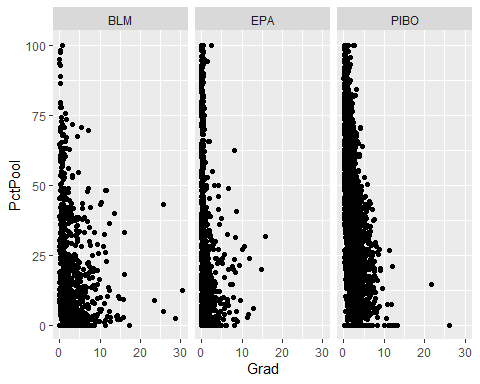
\includegraphics{Sharing_instream_tributary_habitat_data_BAP_files/figure-latex/unnamed-chunk-10-1.pdf}

\begin{Shaded}
\begin{Highlighting}[]
\NormalTok{data }\OperatorTok
\StringTok{  }\KeywordTok{group_by}\NormalTok{(Program) }\OperatorTok
\StringTok{  }\KeywordTok{summarize}\NormalTok{(}\KeywordTok{mean}\NormalTok{(PctPool, }\DataTypeTok{na.rm=}\NormalTok{T))}
\end{Highlighting}
\end{Shaded}

\begin{verbatim}
## # A tibble: 3 x 2
##   Program `mean(PctPool, na.rm = T)`
##   <fct>                        <dbl>
## 1 BLM                           17.6
## 2 EPA                           25.3
## 3 PIBO                          38.0
\end{verbatim}

\begin{Shaded}
\begin{Highlighting}[]
\KeywordTok{ggplot}\NormalTok{(data, }\KeywordTok{aes}\NormalTok{(PctPool))}\OperatorTok{+}\KeywordTok{geom_histogram}\NormalTok{()}\OperatorTok{+}\KeywordTok{facet_wrap}\NormalTok{(}\OperatorTok{~}\NormalTok{Program)}
\end{Highlighting}
\end{Shaded}

\begin{verbatim}
## `stat_bin()` using `bins = 30`. Pick better value with `binwidth`.
\end{verbatim}

\begin{verbatim}
## Warning: Removed 840 rows containing non-finite values (stat_bin).
\end{verbatim}

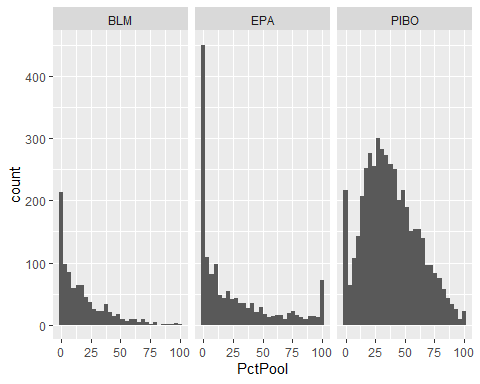
\includegraphics{Sharing_instream_tributary_habitat_data_BAP_files/figure-latex/unnamed-chunk-12-1.pdf}

\begin{Shaded}
\begin{Highlighting}[]
\CommentTok{#library(shiny)}

\CommentTok{#h = ggplot(data, aes(PctPool))+geom_histogram()}

\CommentTok{# Define UI for application that draws a histogram}
\CommentTok{#ui <- fluidPage(}

  \CommentTok{# App title ----}
  \CommentTok{#titlePanel("Pools"),}

  \CommentTok{# Sidebar layout with input and output definitions ----}
  \CommentTok{#sidebarLayout(}

    \CommentTok{# Sidebar panel for inputs ----}
   \CommentTok{# sidebarPanel(}

      \CommentTok{# Input: Slider for the number of bins ----}
    \CommentTok{#  sliderInput(inputId = "bins",}
     \CommentTok{#             label = "Number of bins:",}
      \CommentTok{#            min = min(data$PctPool, na.rm=T),}
       \CommentTok{#           max = max(data$PctPool, na.rm=T),}
        \CommentTok{#          value = 10)}

    \CommentTok{#),}

    \CommentTok{# Main panel for displaying outputs ----}
\CommentTok{#    mainPanel(}

      \CommentTok{# Output: Histogram ----}
 \CommentTok{#     plotOutput(outputId = "h")}
\CommentTok{#}
 \CommentTok{# )}
\CommentTok{#)}

\CommentTok{#ui}
\end{Highlighting}
\end{Shaded}


\end{document}
